\section{Surface Density Distributions}

One measure of surface activity is the spatial distribution of molecules in the interfacial region. The density distribution of both \wat~and \suldiox~were calculated for the equilibrium MD simulations, and the results are presented in figure \ref{fig:density} for both the neat-water and saturated simulations. The \suldiox~in the neat-water system remained at the top slab surface. The \suldiox~in the saturated system accumulated mostly at the surface, but some residual \suldiox~remained in the bulk.

%The density distributions of the \suldiox~were fit to gaussian lineshapes as shown in equation \ref{eq:gaussian} using the common definitions of the variables $A$, $\mu$, and $\sigma$, and given as a function of the distance to the top surface, $z$.

%\begin{equation}
%  \rho(z)=\frac{A}{\sqrt{2 \pi \sigma^2}} e^{-\frac{(z-\mu)^2}{2\sigma^2}}
%  \label{eq:gaussian}
%\end{equation}

In the neat-water slab, the \suldiox~distribution shows a surface affinity when in a low-concentration environment. It does not reside in the bulk or move out of the surface into the gas phase. This surface active behavior was found experimentally by the SFG study by our group,\cite{Tarbuck2005,Tarbuck2006} and also verified by the computational simulations and spectral calculations of Baer et al.\cite{Baer2010} The water behavior hypothesized from the experimental analysis is that a surface \suldiox~hydrate complex forms, and it modifies the structure of water above the Gibbs dividing surface (GDS). \wat~free-OH oscillators are thus shifted in towards the bulk, creating a stronger hydrogen-bonding network. In a later section of this article we look at the effect of \suldiox~on surface water orientation.

Both saturated \suldiox~surfaces exhibit accumulations of \suldiox. However, unlike the neat-water slab, the saturated slab has a non-zero bulk concentration of \suldiox~that does not adsorb to the surface. The added concentration of \suldiox~creates a layer of molecules bound to the top of the water surface. The center of the \suldiox~density distribution is further into the gas phase than for the neat-water surface with a single-\suldiox~molecule. The accumulation of \suldiox~in this classical simulation coincides with the experimental conclusions of \suldiox~surface hydrate complex formation. However, without simulating breakble bonds the chemistry that may pull \suldiox~into the bulk water phase, and the subsequent reaction to form ions is absent. We have confidence in the surface complexation that is exhibited, the effect of the \suldiox~on the surface water molecules, and the accumulation of \suldiox~at the interface. However, we do not yet conclude that the specific locations of \suldiox~on top of the water surface are as accurate as those found in the DFT ab initio calculations of Dang et al.\cite{Baer2010} As was pointed out in their computations, the classical potential does not reproduce the bonding of the first hydration shell around \suldiox, and so conclusions about specific complex formation or geometries are best made from the ab initio simulation results reported.

\begin{figure}[h!]
	\begin{center}
		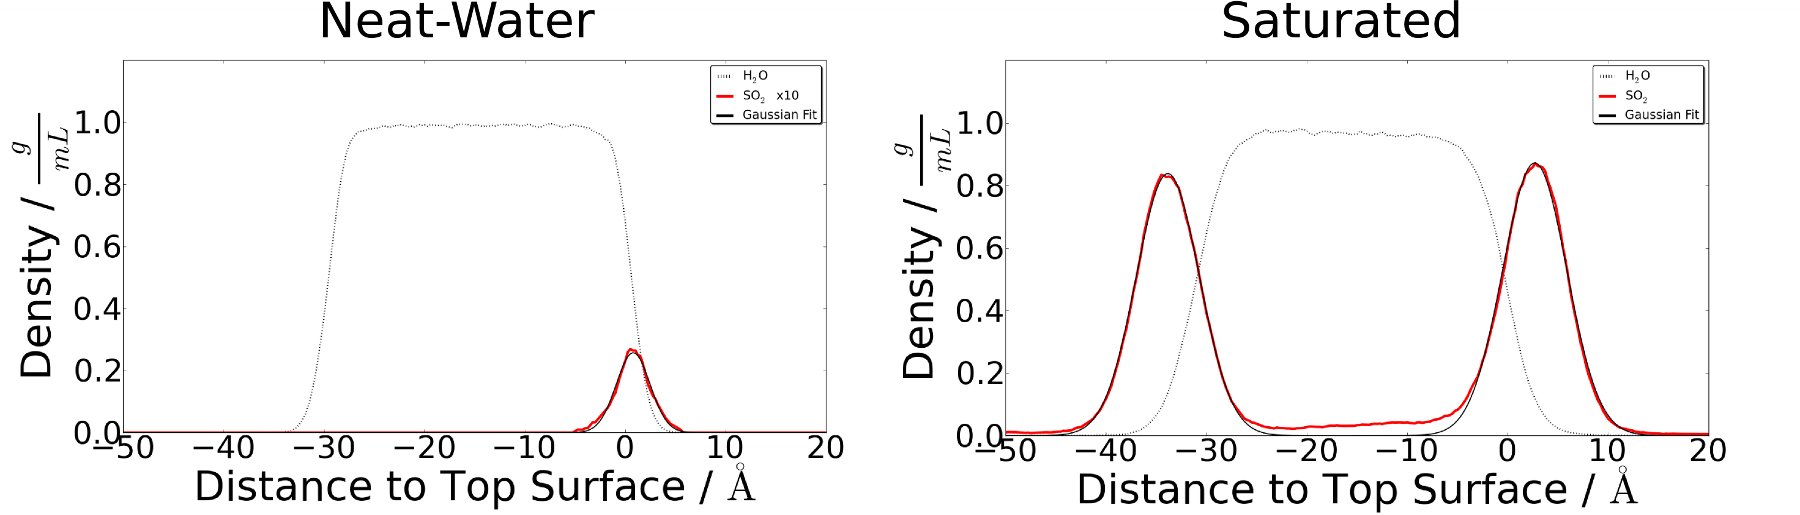
\includegraphics[scale=1.0]{images/density/density.png}
		\caption{Molecular density distributions of \wat~and \suldiox~calculated along the long-axis of the simulated cells. The distance axis shows the distance of the given molecule from the top surface of the \wat~slab, with positive values located above the slab towards the gas phase, and negative values located in the water bulk. The lower slab surface is located at approx. -30\angs. Distributions of both the neat-water simulation with a single \suldiox~(left, scaled 10x for clarity), and the saturated system (right) are shown.}
		\label{fig:density}
	\end{center}
\end{figure}
